
\section{Computational tools}

\subsection{MOOSE}

% intro
\gls{MOOSE}\cite{gaston_moose_2009} is a computational framework that supports engineering analysis applications.
In a nuclear reactor, several partial differential equations describe the physical behavior.
These equations are typically nonlinear, and they are often strongly coupled to each other.
\gls{MOOSE} targets such systems and solves them in a fully coupled manner.

% more details about MOOSE
\gls{MOOSE} is an open-source code under a \gls{LGPL}.
The code itself relies on LibMesh \cite{kirk_libmesh_2006}, an LGPL finite element library, and PetSc, a \gls{BSD}-licensed toolkit for solving nonlinear equations \cite{balay_petsc_2016}.
MOOSE applications define weak forms of the governing equations and 
modularize the physics expressions into "Kernels."
Kernels are C++ classes containing methods for computing the residual and Jacobian contributions of individual pieces of the governing equations.
\gls{MOOSE} and LibMesh translate them into residual and Jacobian functions.
These functions become inputs into PetSc solution routines.

\gls{MOOSE} utilizes the mathematical structure present in \gls{JFNK} methods \cite{knoll_jacobian-free_2004}.
\gls{JFNK} methods are synergistic combinations of Newton-type methods for superlinearly convergence of nonlinear equations and Krylov subspace methods for solving the Newton correction equations.
The Jacobian-vector product links the two methods.
JFNK methods compute such products approximately without forming and storing the elements of the true Jacobian.
The ability to perform a Newton iteration without forming the Jacobian gives JFNK methods potential for application throughout problems governed by nonlinear partial differential equations.

All the software built on the MOOSE framework shares a joint base code.
The applications, by default, utilize monolithic and implicit methods.
This feature facilitates relatively easy coupling between different phenomena and allows for great flexibility, even with a great variance in time scales \cite{novak_pronghorn_2018}.
Additionally, all codes use \gls{MPI} for parallel communication and allow deployment on massively-parallel cluster-computing platforms.

\subsection{Moltres}

\textit{Moltres} \cite{lindsay_introduction_2018} is a MOOSE-based application initially designed for modeling fluid-fuelled \glspl{MSR}.
This simulation tool is open source and operates with an LGPL.
It uses \textit{git} for version control, emphasizing its openness and promoting quality through peer review.

Moltres solves arbitrary-group neutron diffusion, precursors, and temperature governing equations.
It can solve the equations in a fully-coupled way or solve each system independently, allowing for great flexibility and making it applicable to a wide range of nuclear engineering problems.

\subsection{Serpent}

The Serpent Monte Carlo code \cite{leppanen_development_2007} \cite{leppanen_calculation_2014} is a three-dimensional continuous-energy neutron transport code developed by the VTT Technical Research Centre of Finland, and it has been in public distribution since 2009.
Monte Carlo neutron transport codes have several reactor physics applications related to criticality safety analyses, radiation shielding problems, detector modeling, and validation of deterministic transport codes.
The Monte Carlo method's main advantage is its capability to model geometry and interaction physics without significant approximations.
The main disadvantage is that simulating complex systems is computing-intensive, restricting applications to some extent.

Serpent serves two primary purposes: (1) reactor modeling, and (2) group constant generation.
In reactor modeling, the Monte Carlo simulation itself represents the solution to the full-scale problem.
In group constant generation, the transport simulation produces input parameters for a deterministic code.
Based on a few groups, deterministic codes allow for carrying out coupled full-core analyses.

In this work, Serpent produces group constants that serve as an input for Moltres and solves the heterogeneous system.
This last step provides the reference solutions for the validation of the Moltres calculation scheme.
We used Serpent 2.1.31 and the cross-section library JEFF3.1.2 for the calculations.
The reason for using Serpent to generate cross-sections is due to its ability to run explicit simulations of randomly located TRISO particles.
Applying a simple volume homogenization proves inaccurate due to the resonant self-shielding effect of the kernel and coated layers.
Although the particles' explicit modeling is time-consuming, costly, and impractical for most applications, it is necessary.

\section{Mathematical basis}

\subsection{Diffusion and precursors equations}

% Neutronics
Equations \ref{eq:diffusion} and \ref{eq:precursors} describe the time dependent behavior of the neutronics.

\begin{align}
  % diffusion
  \frac{1}{v_g}\frac{\partial}{\partial t} \phi_g &= \nabla \cdot D_g \nabla \phi_g -
  \Sigma_g^r \phi_g + \sum_{g \ne g'}^G \Sigma_{g'\rightarrow g}^s \phi_{g'} +
  \chi_g^p \sum_{g' = 1}^G (1 - \beta) \nu \Sigma_{g'}^f \phi_{g'} +
  \chi_g^d \sum_i^I \lambda_i C_i \label{eq:diffusion} \\
  % precursors
  \frac{\partial}{\partial t} C_i &= \sum_{g'= 1}^G \beta_i \nu \Sigma_{g'}^f \phi_{g'} - \lambda_i C_i
  \label{eq:precursors}
        \intertext{where}
        v_g &= \mbox{group $g$ neutron speed} \notag \\
        \phi_g &= \mbox{group $g$ neutron flux} \notag \\
        t &= \mbox{time} \notag \\
        D_g &= \mbox{group $g$ diffusion coefficient} \notag \\
        \Sigma_g^r &= \mbox{group $g$ macroscopic removal cross-section} \notag \\
        \Sigma_{g'\rightarrow g}^s &= \mbox{group $g'$ to group $g$ macroscopic scattering cross-section} \notag \\
        \chi_g^p &= \mbox{group $g$ prompt fission spectrum} \notag\\
        G &= \mbox{number of discrete energy groups} \notag \\
        \nu &= \mbox{number of neutrons produced per fission} \notag \\
        \Sigma_g^f &= \mbox{group $g$ macroscopic fission cross-section} \notag \\
        \chi_g^d &= \mbox{group $g$ delayed fission spectrum} \notag \\
        I &= \mbox{number of delayed neutron precursor groups} \notag \\
        \beta &= \mbox{delayed neutron fraction} \notag \\
        \lambda_i &= \mbox{average decay constant of delayed neutron precursors in precursor group $i$} \notag \\
        C_i &= \mbox{concentration of delayed neutron precursors in precursor group $i$.} \notag \\
\end{align}

% Boundary conditions
We apply the vacuum boundary condition to the diffusion equation.
The vacuum boundary condition states that no neutrons penetrate the boundary in the inward direction.
In other words, the incoming current density ($J^-(r_s, t)$) is equal to zero, equation \ref{eq:vacuumbc1} \cite{duderstadt_nuclear_1976}.

\begin{align}
   J^-(r_s, t) = \frac{1}{4} \phi(r_s, t) + \frac{D}{2} \hat{n_s} \cdot \nabla \phi (r_s, t) = 0
\label{eq:vacuumbc1}
\end{align}

\subsection{Thermal-hydraulics}
\label{ch3:th}

The governing equation for the temperature of the solids is the three-dimensional heat conduction equation \cite{melese_thermal_1984}.
Equations \ref{eq:tempsolid} to \ref{eq:heatsource2} allow for solving the temperature in the fuel, moderator, and reflector.

\begin{align}
    \rho_i c_{p,i} \frac{\partial}{\partial t} T_i &= k_i \nabla^2 T_i + Q_i \label{eq:tempsolid} \\
    Q_f &= \sum_{g = 1}^{G} \epsilon_g^f \Sigma_g^f \phi_g \label{eq:heatsource} \\
    Q_m &= Q_r = 0 \label{eq:heatsource2}
  \intertext{where}
  i &= \mbox{f (fuel), m (moderator), r (reflector)} \notag \\
  \rho_i &= \mbox{material $i$ density} \notag \\
  c_{p,i} &= \mbox{material $i$ heat capacity} \notag \\
  k_i &= \mbox{material $i$ thermal conductivity } \notag \\
  T_i &= \mbox{material $i$ temperature} \notag \\
  Q_i &= \mbox{material $i$ volumetric heat source} \notag \\
  \epsilon_g^f &= \mbox{energy released per fission} \notag \\
  \Sigma_g^f &= \mbox{group $g$ macroscopic fission cross-section} \notag \\
  \phi_g &= \mbox{group $g$ neutron flux.} \notag
\end{align}

% coolant
% section 2-5.2 white_viscous_2006
% equations 8-10 tak_practical_2012
The governing equation of the coolant is the one-dimensional form of the continuity, momentum, and energy conservation equations, equations \ref{eq:continuity} to \ref{eq:convection} \cite{white_viscous_2006}\cite{tak_practical_2012}.

\begin{align}
 	\frac{\partial}{\partial t} \rho_c + \nabla \cdot (\rho_c u) &= 0 \label{eq:continuity} \\
  \rho_c \left(\frac{\partial}{\partial t} u + u\frac{\partial}{\partial z}u \right) &= - \frac{\partial}{\partial z}p - \tau \frac{\varepsilon}{A} - \rho_c g \label{eq:momentum} \\
 	\rho_c \left( \frac{\partial}{\partial t} (c_{p,c} T_c) + u\frac{\partial}{\partial z} (c_{p,c} T_c) \right) &= \frac{\partial}{\partial t} p + u\frac{\partial}{\partial z} p +  q'''_{conv} 	\label{eq:tempcool} \\
  \tau &= \frac{f}{2} \rho_c u^2 \label{eq:friction} \\
  q'''_{conv} &= h\frac{\varepsilon}{A} (T_i-T_c) \label{eq:convection}
  \intertext{where}
  \rho_c &= \mbox{coolant density} \notag \\
  u &= \mbox{coolant velocity} \notag \\
  p &= \mbox{coolant pressure} \notag \\
  \tau &= \mbox{shear stress} \notag \\
  \varepsilon &= \mbox{wetted perimeter} \notag \\
  A &= \mbox{cross-sectional area} \notag \\
  g &= \mbox{gravity} \notag \\
  c_{p,c} &= \mbox{coolant specific heat capacity} \notag \\
  T_c &= \mbox{coolant temperature} \notag \\
  k_c &= \mbox{coolant thermal conductivity} \notag \\
  q'''_{conv} &= \mbox{convective heat transfer} \notag \\
  f &= \mbox{friction factor} \notag \\
  h &= \mbox{heat transfer coefficient} \notag \\
  T_i &= \mbox{solid temperature.} \notag
\end{align}

\section{OECD/NEA MHTGR-350 MW Benchmark}

The deterministic neutronic thermal-fluids and transient analysis methods available for prismatic \glspl{HTGR} lag behind the state-of-the-art technologies of other reactors.
This delay has motivated the development of more accurate tools for the design and safety evaluations of \glspl{HTGR}.
In addition to the development of new methods, it is essential to define appropriate benchmarks to compare these new methods' capabilities.
The \gls{OECD}/\gls{NEA} defined such a benchmark \cite{oecd_nea_benchmark_2017} using the \gls{MHTGR}-350 MW reactor \cite{silady_licensing_1988} as the reference design.
The scope of the benchmark is twofold: (1) establish a well-defined problem, based on a common given data set, to compare methods and tools in core simulation and thermal fluids analysis, and (2) test the depletion capabilities of various lattice physics codes available for prismatic \glspl{HTGR}.

The benchmark defines several Phases and Exercises:

\begin{itemize}
        \item Phase I: Steady State
        \begin{enumerate}
            \item Neutronics solution with fixed cross-sections. 
            \item Thermal fluids solution with given heat sources.
            \item Coupled neutronics-thermal fluids steady state solution.
        \end{enumerate}

        \item Phase II: Transient Cases
        \begin{enumerate}
            \item Depressurized Conduction Cooldown without reactor trip.
            \item Pressurized Conduction Cooldown with reactor trip.
            \item Water ingress with reactor trip.
            \item Power 100-80-100 load follow.
        \end{enumerate}

        \item Phase III: Lattice Depletion Case
\end{itemize}

\section{MHTGR-350 Reactor Description}

This section describes the \gls{MHTGR}-350 reactor.
Table \ref{tab:maincharac} lists its main characteristics.
The core consists of an array of hexagonal fuel elements in a cylindrical arrangement, Figure \ref{fig:layout}.
Nineteen graphite replaceable reflector elements compose the inner reflector region.
A ring of identically sized graphite replaceable reflector elements surrounds the fuel elements.
Then, a region of permanent reflector elements follows the replaceable reflectors.
The reactor vessel encases all the elements.

\begin{table}[htbp!]
  \centering
    \caption{MHTGR-350 Characteristics \cite{oecd_nea_benchmark_2017}.}
  \begin{tabular}{ll}
  \toprule
  Characteristics                   & Value               \\ \midrule
  Installed Thermal Capacity        & 350 MWt             \\
  Installed Electric Capacity       & 165 MWe             \\
  Core inlet/outlet Temperature     & 259/687$^{\circ}$C  \\
  Power Density                     & 5.9 MW/m$^3$        \\
  Reactor Vessel Outside diam.      & 6.8 m               \\
  Reactor Vessel Height             & 22 m                \\
  Active core radius                & 2.97 m              \\
  Active core height                & 7.93 m              \\
  Top reflector height              & 1.20 m              \\
  Bottom reflector height           & 1.60 m              \\
  Number of fuel columns            & 66                  \\
  Number of inner reflector columns & 19                  \\
  Number of outer reflector columns & 78                  \\
  \bottomrule
  \end{tabular}
  \label{tab:maincharac}
\end{table}

\begin{figure}[htbp!]
    \centering
    \subfloat[Core radial layout. Image reproduced from \cite{oecd_nea_benchmark_2017}.]{
        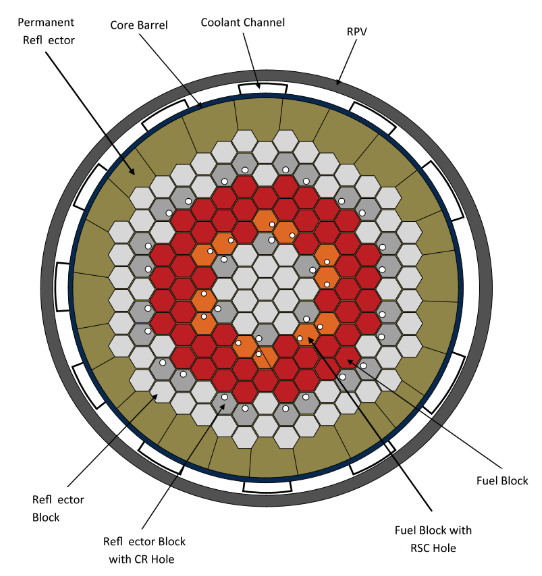
\includegraphics[width=0.45\textwidth]{figures/radial-layout.png}
    }
    \subfloat[Core axial layout. Image reproduced from \cite{oecd_nea_benchmark_2017}.\label{fig:layoutb}]{
        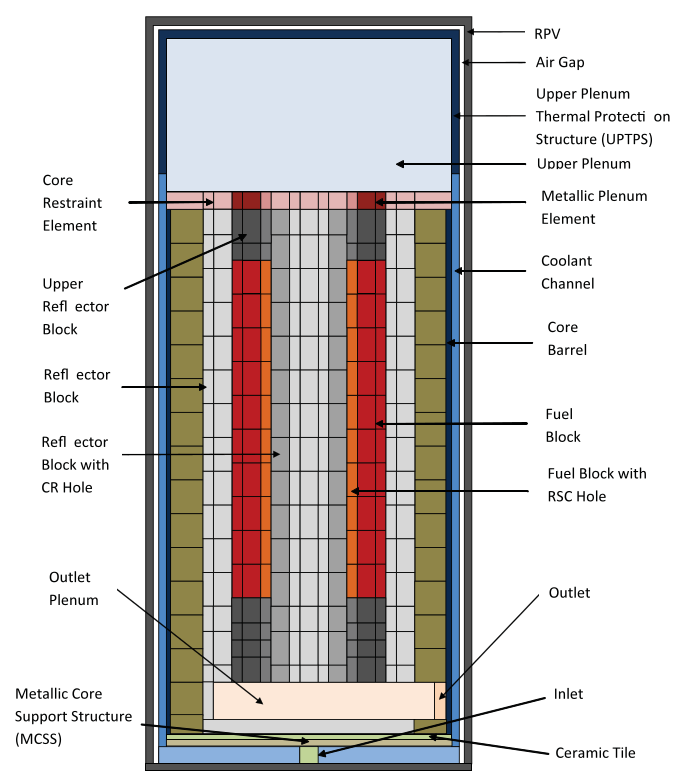
\includegraphics[width=0.45\textwidth]{figures/axial-layout.png}
    }
    \hfill
    \caption{MHTGR reactor layout.}
    \label{fig:layout}
\end{figure}

% \begin{figure}[htbp!]
%   \centering
%   \begin{subfigure}[t]{0.4\textwidth}
%     \centering
%     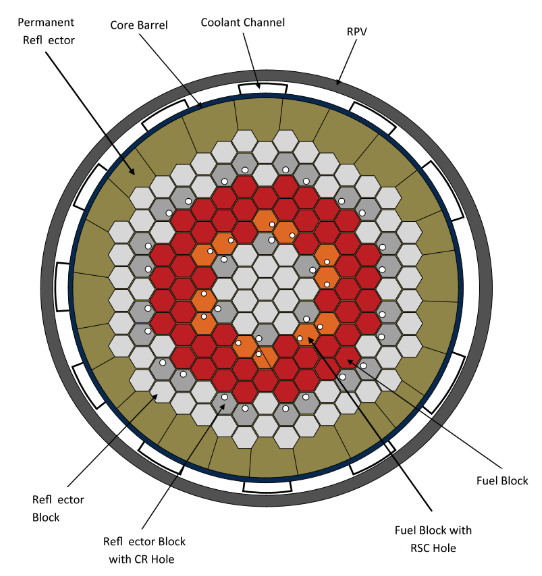
\includegraphics[width=0.95\linewidth]{figures/radial-layout.png}
%     \caption{Core radial layout. Image reproduced from \cite{oecd_nea_benchmark_2017}.}
%   \end{subfigure}
%   \begin{subfigure}[t]{0.4\textwidth}
%     \centering
%     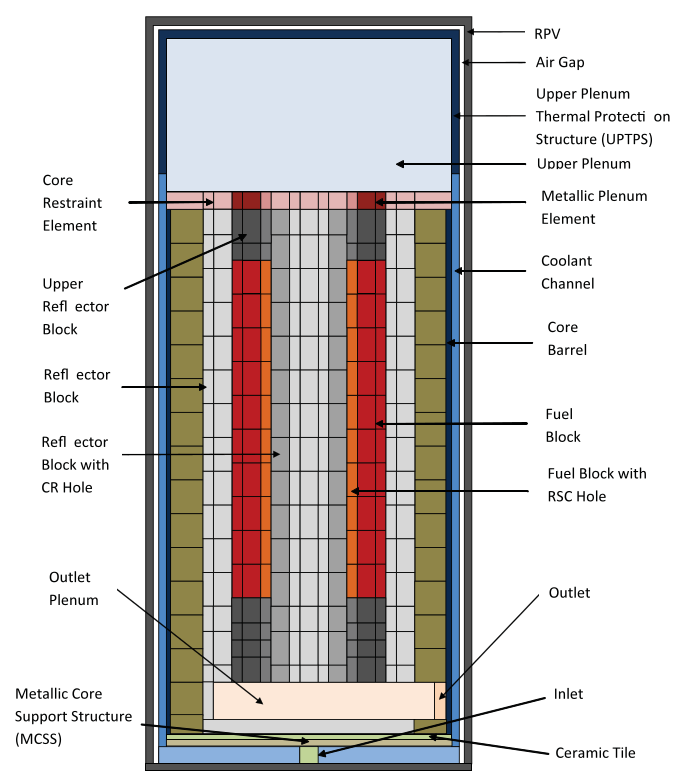
\includegraphics[width=0.95\linewidth]{figures/axial-layout.png}
%     \caption{Core axial layout. Image reproduced from \cite{oecd_nea_benchmark_2017}.}
%     \label{fig:layoutb}
%   \end{subfigure}
%   \hfill
%   \caption{MHTGR reactor layout.}
%   \label{fig:layout}
% \end{figure}

Ten layers of fuel elements stacked on top of each other compose the 66 fuel columns that integrate the active core.
Figure \ref{fig:layoutb} shows an axial view of the reactor.
The core has two types of fuel elements: a standard element and a reserve shutdown element that contains a channel for \gls{RSC}, Figure \ref{fig:fuelassembly}.
Table \ref{tab:element-characteristics} specifies the details of the MHTGR-350 fuel elements.
Twelve columns in the core contain \gls{RSC} channels for reserve shutdown borated graphite pellets.
Hoppers above the core house the pellets, and if the \glspl{CR} become inoperable, the pellets drop into the channels \cite{oecd_nea_benchmark_2017}.

\begin{figure}[htbp!]
  \centering
    \subfloat[Standard fuel assembly. Image reproduced form \cite{tak_numerical_2008}.]{
        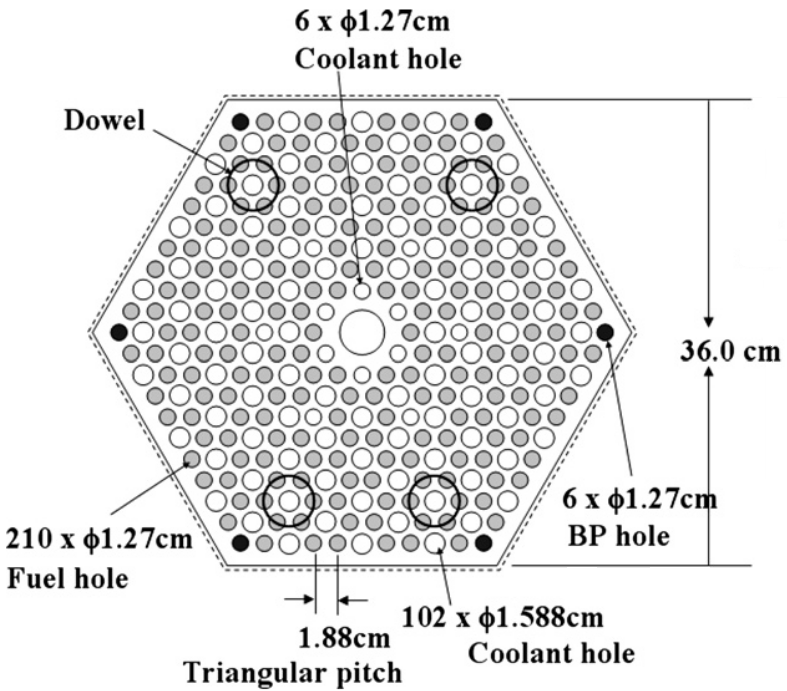
\includegraphics[width=0.45\textwidth]{figures/fuel-assembly}
    }
    \subfloat[RSC fuel assembly. Image reproduced form \cite{tak_practical_2012}.]{
        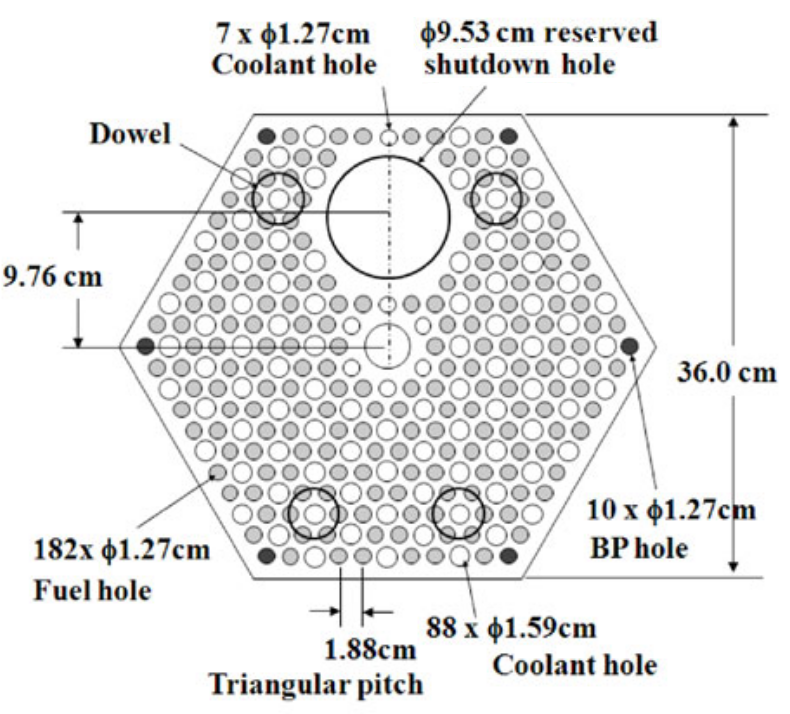
\includegraphics[width=0.45\textwidth]{figures/fuel-assembly-rsc}
    }
  \hfill
    \caption{MHTGR-350 fuel assembly layout.}
  \label{fig:fuelassembly}
\end{figure}

\begin{table}[htbp!]
\centering
      \caption{MHTGR350 fuel element characteristics \cite{oecd_nea_benchmark_2017}.}
      \label{tab:element-characteristics}
    \begin{tabular}{@{}l S[table-format=2.2] c}
    \toprule
    \multicolumn{1}{c}{Shared characteristics} & \multicolumn{1}{c@{}}{Value} & \multicolumn{1}{c@{}}{Units} \\
    \midrule
  Block pitch (flat-to-flat)       & 36      & cm       \\
  Fuel length                      & 79.3    & cm       \\
  Fuel handling diameter           & 3.5     & cm       \\
  Fuel handling length             & 26.4    & cm       \\
  RSC hole diameter                & 9.525   & cm       \\
  RSC center to assembly center    & 9.756   & cm       \\
  Fuel/coolant pitch               & 1.879   & cm       \\
  Fuel hole radius                 & 0.635   & cm       \\
  Compacts per fuel hole           & \multicolumn{1}{c@{}}{15}    & -        \\
  Large coolant hole radius        & 0.794   & cm       \\
  Small coolant hole radius        & 0.635   & cm       \\
  LBP hole radius                  & 0.635   & cm       \\
  Block graphite density           & 1.85    & g/cm$^3$ \\
  \midrule

      \multicolumn{1}{c}{Standard element} &  &  \\

  \midrule
  Number of large coolant holes    & \multicolumn{1}{c@{}}{120}   & -        \\
  Number of small coolant holes    & \multicolumn{1}{c@{}}{6}     & -        \\
  Number of fuel holes             & \multicolumn{1}{c@{}}{210}   & -        \\
  \midrule

      \multicolumn{1}{c}{RSC element} &  &  \\

  \midrule
  Number of large coolant holes    & \multicolumn{1}{c@{}}{88}    & -        \\
  Number of small coolant holes    & \multicolumn{1}{c@{}}{7}     & -        \\
  Number of fuel holes             & \multicolumn{1}{c@{}}{186}   & -        \\
    \bottomrule
    \end{tabular}
\end{table}

% Fuel assemblys and triso particles
The fuel elements contain blind holes for fuel compacts and full-length channels for helium coolant flow.
Table \ref{tab:compact} specifies the details of the TRISO particle and fuel compact designs of the \gls{MHTGR}-350.

\begin{table}[htbp!]
\centering
    \caption{TRISO and fuel compact characteristics \cite{oecd_nea_benchmark_2017}.}
    \label{tab:compact}
    \begin{tabular}{@{}l S[table-format=2.1] c}
    \toprule
    \multicolumn{1}{c}{Characteristic} & \multicolumn{1}{c@{}}{Value} & \multicolumn{1}{c@{}}{Units} \\
    \midrule
  Fuel                             & UC$_{0.5}$O$_{1.5}$   & -        \\
  Enrichment (average)             & 15.5                  & wt\%     \\
  Packing fraction (average)       & 0.35                  & -        \\
  Kernel radius                    & 0.02125               & cm       \\
  Buffer radius                    & 0.03125               & cm       \\
  IPyC radius                      & 0.03475               & cm       \\
  SiC radius                       & 0.03825               & cm       \\
  OPyC radius                      & 0.04225               & cm       \\
  Compact radius                   & 0.6225                & cm       \\
  Compact gap radius               & 0.6350                & cm       \\
  Compact length                   & 4.9280                & cm       \\
  Kernel density                   & 10.50                 & g/cm$^3$ \\
  Buffer density                   & 1.00                  & g/cm$^3$ \\
  IPyC density                     & 1.90                  & g/cm$^3$ \\
  SiC density                      & 3.20                  & g/cm$^3$ \\
  OPyC density                     & 1.90                  & g/cm$^3$ \\
  Compact matrix density           & 1.74                  & g/cm$^3$ \\
    \bottomrule
    \end{tabular}
\end{table}

% Reactivity control
A combination of \gls{LBP} and \glspl{CR} controls the core reactivity.
The \gls{LBP} consists of \gls{B4C} granules dispersed in graphite compacts.
The current design uses six \gls{LBP} rods per element.
Table \ref{tab:LBP} displays the characteristics of the \gls{LBP} compacts.
The reactor has 30 \glspl{CR}.
Six of them are start-up \glspl{CR}, and their location is the inner reflector.
The remaining 24 are operating \glspl{CR} and control the reactivity during power operation and a reactor trip.

\begin{table}[htbp!]
\centering
    \caption{LBP compact characteristics \cite{oecd_nea_benchmark_2017}.}
    \label{tab:LBP}
    \begin{tabular}{@{}l S[table-format=1.4] c}
    \toprule
    \multicolumn{1}{c}{Characteristic} & \multicolumn{1}{c@{}}{Value} & \multicolumn{1}{c@{}}{Units} \\
    \midrule
  Absorber                         & B$_{4}$C              & -         \\
  Packing fraction                 & 0.109                 & -         \\
  Kernel radius                    & 0.0100                & cm        \\
  Buffer radius                    & 0.0118                & cm        \\
  PyC radius                       & 0.0141                & cm        \\
  Compact radius                   & 0.5715                & cm        \\
  Compact gap radius               & 0.6350                & cm        \\
  Rod length                       & 72.187                & cm        \\
  Kernel density                   & 2.47                  & g/cm$^3$  \\
  Buffer density                   & 1.00                  & g/cm$^3$  \\
  PyC density                      & 1.87                  & g/cm$^3$  \\
  Compact matrix density           & 0.94                  & g/cm$^3$ \\
    \bottomrule
    \end{tabular}
\end{table}
